\documentclass[10pt,conference,compsoc]{IEEEtran}
\special{papersize=8.5in,11in}

\usepackage[utf8]{inputenc}
\usepackage{graphicx}
\usepackage{epstopdf}
\usepackage{subfig}
\usepackage{bm}
\usepackage{url}
\usepackage{lipsum}
\usepackage{amsmath}
\usepackage{amssymb}
\usepackage{booktabs}
\usepackage[ruled,noend,noline]{algorithm2e}
\usepackage[pass]{geometry}

\begin{document}

%*******************************************************************************
% Title and Authors
%*******************************************************************************
\title{Criminal link mining in data stream environment}

% author names and affiliations
% use a multiple column layout for up to three different
% affiliations
%\author{
%\IEEEauthorblockN{Michael Shell}
%\IEEEauthorblockA{School of Electrical and\\Computer Engineering\\
%Georgia Institute of Technology\\
%Atlanta, Georgia 30332--0250\\
%Email: http://www.michaelshell.org/contact.html}
%\and
%\IEEEauthorblockN{Homer Simpson}
%\IEEEauthorblockA{Twentieth Century Fox\\
%Springfield, USA\\
%Email: homer@thesimpsons.com}
%\and
%\IEEEauthorblockN{Giacomo Marciani and Michele Porretta}
%\IEEEauthorblockA{Department of Civil Engineering and Computer Science Engineering\\
%University of Rome Tor Vergata, Italy\\
%Email:\{gmarciani, mporretta\}@acm.org\\}}

\author{\IEEEauthorblockN{Giacomo Marciani}
\IEEEauthorblockA{Department of Civil Engineering\\and Computer Science Engineering\\
University of Rome Tor Vergata\\ Rome, Italy\\
Email: gmarciani@ieee.org}
\and
\IEEEauthorblockN{Michele Porretta}
\IEEEauthorblockA{Department of Civil Engineering\\and Computer Science Engineering\\
University of Rome Tor Vergata\\ Rome, Italy\\
Email: mporretta@acm.org}
\and
\IEEEauthorblockN{Matteo Nardelli}
\IEEEauthorblockA{Department of Civil Engineering\\and Computer Science Engineering\\
University of Rome Tor Vergata\\ Rome, Italy\\
Email: nardelli@ing.uniroma2.it}}

% make the title area
\maketitle

% correct bad hyphenation here
\hyphenation{op-tical net-works semi-conduc-tor}

% no keywords

\IEEEpeerreviewmaketitle

%*******************************************************************************
% Content
%*******************************************************************************
\begin{abstract}
This paper provides a sample of a \LaTeX\ document which conforms,
somewhat loosely, to the formatting guidelines for
ACM SIG Proceedings. It is an {\em alternate} style which produces
a {\em tighter-looking} paper and was designed in response to
concerns expressed, by authors, over page-budgets.
It complements the document \textit{Author's (Alternate) Guide to
Preparing ACM SIG Proceedings Using \LaTeX$2_\epsilon$\ and Bib\TeX}.
This source file has been written with the intention of being
compiled under \LaTeX$2_\epsilon$\ and BibTeX.

The developers have tried to include every imaginable sort
of ``bells and whistles", such as a subtitle, footnotes on
title, subtitle and authors, as well as in the text, and
every optional component (e.g. Acknowledgments, Additional
Authors, Appendices), not to mention examples of
equations, theorems, tables and figures.

To make best use of this sample document, run it through \LaTeX\
and BibTeX, and compare this source code with the printed
output produced by the dvi file. A compiled PDF version
is available on the web page to help you with the
`look and feel'.
\end{abstract}

\section{Introduction}
\label{sec:introduction}

The data-driven fight against organized crime is opening new research challenges and directions. 
In this context, it is necessary to develop big data analytics systems leveraging social network analysis models that are both aware of criminological assumptions and ready to be executed in a data stream environment.

In this work we focus on link detection and prediction, namely the task of determining existent though invisible inetractions, and the prediction of future ones \cite{Hasan2011}.
Currently, these problems are a long-standing challenge in modern information science, and the mainstream solutions leverages algorithms based on 
\textit{structural metrics} and \textit{statistical models} \cite{Liben-Nowell,Lu2011}.

%In this era it is necessary to develop even more efficient big data technologies and stream-aware topological models.
%In particular, the real-time discovery of hidden criminal patterns is an outstanding challenge for security and law enforcement agencies.

%The \textit{social network analysis (SNA)} is an interdisciplinary field from social sciences, statistics, graph theory and computer science. SNA has received considerable attention from the scientific community, in order to find algorithmic solutions to extract missing information, identify hidden interactions between individuals, and so on.
 
%There are many domains that can be represented with a social network and to do that on network analysis, for example social interactions between people, biological interaction between proteins, systems informations. An additional field of application relates to criminal networks, to facilitate the authorities in the investigation of organized crime, such as terrorism, drug trafficking, fraud, armed gang crimes and others\cite{xu2005criminal}.

%The analysis on large volumes of data produced by a criminal network, such as phone records, bank transitions, interceptions, sales of weapons or vehicles, and more, significantly reduces the raw data and provides the mechanisms to study the structural hidden properties of network\cite{xu2005criminal}.

%In this paper, we focus on a criminal scenario and describe it on a graph where apply the link mining techniques. In particular, we want to predict the likelihood that a link, between two entities, is hidden or that may arise in the future. These problems are called respectively the \textit{link detection problem} and \textit{link prediction problem}. 

The remainder of the paper is organized as follows:
Section~\ref{sec:background} gives the background, useful to better understand our work;
Section~\ref{sec:data-model} defines the data model adopted to describe criminal entities and interactions;
Section~\ref{sec:link-detection} and Section~\ref{sec:link-prediction} defines the proposed local metrics for link detection and prediction;
Section~\ref{sec:architecture} shows the data stream processing architecture to deploy these metrics;
Section~\ref{sec:metrics-update} shows the data stream algorithm to detect the necessary metrics updates in a data stream processing environment.
Section~\ref{sec:evaluation} gives the experimental results about the performance achieved with the proposed metrics;
Section~\ref{sec:further-improvements} outlines the possible improvements for the proposed metrics;
Section~\ref{sec:conclusions} concludes this article, summarizing our work and results.

\section{Background}
\label{sec:background}

We assume that the reader is familiar with the fundamentals of graph theory. 
However, we make a brief recap to introduce what we will see in the next sections.

Let $G(V,E,w)$ be an undirected weighted graph, where $V$ is the set of vertices, $E$ is the set of edges and $w:E\rightarrow\Re$ is the weight function. 
A \textit{path} $\pi_{x,y}$ between two vertices $x$,$y$ of \textit{length} $k$ in $G$ is a sequence of vertices $v_{1},v_{2},\ldots,v_{k}$, where $x = v_{1}$ and $y = v_{k}$, such that the edge $(v_{i},v_{i+1}) \in E$ for $i = 1, 2,\ldots,k-1$. 
The distance $d(x,y)$ between $x$ and $y$, is the length of the shortest path from $x$ to $y$ (or vice versa).
A graph is \textit{connected} if there is a path between every pair of vertices; otherwise, it is not connected and made of at least two \textit{connected components}.
Given two vertices $x,y \in V$, we denote with $\Gamma_{x}$ the set of neighbors of $x$ (i.e. adjacent vertices) and with $\Gamma_{x,y} = \Gamma_{x} \bigcap \Gamma_{y}$ the set of common neighbors between $x$ and $y$.

A criminal network is a social structure made up of related agents sharing some criminal intent.
We represent a criminal network with the graph $G(V,E,w)$, where $v\in V$ represents a person, a group, an assets or a place, and $E$ represents their relations, for which the tipology and relevance are encapsulated by the correspondent weight.  

% sostituito dalle due frasi precedenti
%with the topological structure of a network, in which each node $v \in V$ is an individual or an organization, and each edge $e=(u,v)\in E$ represents a link (i.e. an interaction) between two nodes, $u$ and $v$. 

% INSERIRE DEFINIZIONE DI LINK MINING, LINK DETECTION E PREDICTION

% inserirei nella introduzione, perchè non è un background, ma la spiegazione di ciò di cui ci occupiamo
%In this paper, we focus on a criminal scenario and describe it on a graph where apply the link mining techniques. In particular, we want to predict the likelihood that a link, between two entities, is hidden or that may arise in the future. These problems are called respectively the \textit{link detection problem} and \textit{link prediction problem}. 

% da inserire nella definizione di link detection e prediction (sopra)
%Briefly, we refer to the first case when the link between two nodes may already exist, but not visible, while we refer to the second case to indicate the prediction of future interaction between two observed individuals\cite{Hasan2011}.

% lo inserirei nella evaluation
%Formally, for two istants $t$ and $t' > t$, we denote $G[t,t']$ the subgraph of G consisting of all edges with a timestamp between $t$ and $t'$. Identified four times: $t_{0}, t'_{0}, t_{1}, t''_{1}$, with $t_{0}<t'_{0}<t_{1}<t'_{1}$, we refer to $[t_{0},t'_{0}]$ as the \textit{training interval} and $[t_{1},t'_{1}]$ as the \textit{test interval}. Applying a \textit{prediction algorithm} on the graph obtained after the training interval, as $G[t_{0},t'_{0}]$, we want to make a prediction on the edges that will be present in the graph $G[t_{1},t'_{1}]$ and not present in $G[t_{0},t'_{0}]$\cite{Liben-Nowell}.
%In this work, the notions of training interval and test interval, are provided with the only purpose to test the algorithm that will be presented in the following. After all, this application produce an output of links mining in real time: in which each instant $t\textsuperscript{*}>t_{0}$ identifies a graph $G[t_{0},t\textsuperscript{*}]$ on which to execute the algorithm. More details about the real time processing are explained in Section \ref{sec:architecture}.

Currently, the problem of link prediction, as the link detection, is a long-standing challenge in modern information science. 
The mainstreaming class of algorithms are the \textit{similarity-based algorithms}. %inserire citazione
Other are based on \textit{Markov chains} or \textit{statistical models}, as extensively discussed in \cite{Liben-Nowell} and \cite{Lu2011}.

%sostituito dalle due frasi precedenti.
%There are many algorithms for this problem and ways to address this challenge. 
%The mainstreaming class of algorithms so-called \textit{similarity-based algorithms}. Other algorithms are based on \textit{Markov chains} or on \textit{statistical models}, as extensively discussed in \cite{Liben-Nowell} and \cite{Lu2011}.

Let us consider the link prediction, because the link detection is analogous, the metrics used for this task are the same adopted: the difference concerns how the results are interpreted. The similarity metrics are so many and they and differ because the size in which focus the analysis. 
In detail, let $s_{x,y}$ the likelihood, i.e. the \textit{score}, as \textit{proximity} or \textit{similarity}, that between the nodes $x$,$y$ there will be a link in the future, provided by the algorithm that implements the similarity considered metric, and let $\pi_{x,y}$ a path between them, we denote \textit{local indices} the metrics that can only compute the $s_{x,y}$ at distance $d_{\pi}(x,y) = 2$ (i.e it's applicable on only nodes that have a common neighbor $\in \Gamma_{x,y}$). 

Other types of metrics are \textit{quasi-local} indices, that consider $d(x,y) \geq t$, where $t\in \mathbb{Z}, t\geq 1 $, as \textit{locality degree}, identifies a neighborhood with a max length equal to $t$ steps, starting from the node $x$ to $y$. 
Quasi-local metrics are a good tradeoff of accuracy and computational complexity, because the global indices require considerable computational effort, while local indexes are limited. 
Another metrics are \textit{global indices}, that computes the score between any pairs of nodes in $G$ not directly connected\cite{Lu2011}. The metrics used in this work are presented in Section~\ref{sec:link-detection,sec:link-prediction}.

% eliminerei questa frase: link detection non è la normalizzazione nè di RA nè di LP. Il fatto che la metrica di link prediction sia la normalizzazione di RA lo scriverei nella sezione di link prediction.
%The metrics that will present in the following Sections~\ref{sec:link-detection,sec:link-prediction}, are a normalized extension of \textit{Resource Allocation Index (RA)} and \textit{Local Path (LP)}\cite{Lu2011,zhou2009predicting,lu2009similarity}.

% leverei la descrizione di RA e LP, lasciando solamente la citazione dell'articolo che ne parla.
%, that we report for simplicity:
%\begin{equation}
%\label{eqn:resource-allocation}
%s_{xy}\textsuperscript{RA} = 
%\sum\limits_{z\in\Gamma_{x,y}}\frac{1}{k_{z}}
%\end{equation}
%where $k_{z}$ is the degree of node $z$.
%
%\begin{equation}
%\label{eqn:local-path}
%s_{xy}\textsuperscript{LP(k)} = 
%A^{2} + \epsilon A^{3} + \epsilon^{2}A^{4}+...+\epsilon^{k-2}A^{k}
%\end{equation}
%where $k\geq 1$ is a locality degree, $A$ is the adjacency matrix, and $\epsilon$ is a free parameter. For example, $A_{xy}^{2}$ is also the number of different paths with length $2$ connecting $x$ and $y$.

% The RA is an local index and LP is a quasi-local index. 
%Both metrics for link prediction assigned to a pair $x$,$y$ a score, representing their possible future relationship. This score can be viewed as a measure of similarity between nodes $x$ and $y$. Notice that for each pair of nodes, $x$, $y \in V$, we have that $s_{xy} = s_{yx}$. Performing an ranking among the RA score on a graph $G$, can be get the top most likely link those still not present in G.

% Da inserire in evaluation
%Some precision indices are usable to evaluate the accuracy of the metric applied, as we shall see in the evaluation section.

% Da inserire in evaluation
%Notice that, in this work we assume that the graph is connected, therefore each pair of nodes is connected by a path. If we had in the case of a not connected graph, with a large connected component, as \textit{giant component}, and other small size connected components, the accuracy would be distorted by different \textit{density} of edges in a connected components.

%Link mining refers to data mining techniques that consider data links when building descriptive or predictive models \cite{getoor2005link}.

\section{Data model}
\label{sec:data-model}

The criminological domain handles a wide variety of entities and relations between them.
When representing a criminal network with a graph theory model, this variety must be addressed.
Nodes and edges should not be limited to represent people and their mutual knowledge, but also places, assets, not yet investigated groups and every kind of interaction between them. 

In this scenario, a generic node should be labeled with an IRI pointing to an external knowledge base.
A generic edge should be undirected and weighted according to the EWMA  relevance of the observed interaction. 

Furthermore, also the investigation dynamics should be considered. Since entities are observed in their interactions, isolated nodes has no sense in this model. This means that a node insertion occurs only through the insertion of an interaction in which it is involved.

Such a general model makes the link mining task more flexible and adaptable to different criminal contexts.
\section{Link detection}
\label{sec:link-detection}

The link detection is the task of discovering \textit{hidden links} in a network. 
A link $(x,y)$ is hidden if it exists in reality, but it is missing because, it has been neglected during investigations or it has been deliberately concelad by criminals.

We present here a local metric for link detection, based on the following criminological assumptions: 
(i) two criminal nodes hide their direct relation interposing some nodes between them, namely \textit{mediator nodes}, 
(ii) these nodes are mainly dedicated to let them interact,
(iii) the greater the number of these nodes, the greater the likelihood of hidden linkage. 

Formally, 
(i) a direct link $(x,y)$ can be hidden by a path $\pi=(x,z_{1},\ldots,z_{h},y)$, where $z_{1},\ldots,z_{h}$ are mediator nodes,
(ii) the interaction weight $w_{z_{i}}$ involving a mediator node $z_{i}$ is mainly dedicated to convey the hidden interaction between $(x,y)$, that is $\frac{w_{x,z_{i}}+w_{z_{i},y}}{w_{z_{i}}} > 1- \frac{w_{x,z_{i}}+w_{z_{i},y}}{w_{z_{i}}}$.

Let us consider an undirected weighted graph $G(V,E,w)$ with $w:E\rightarrow\Re_{\geq1}^{+}$ and a pair of nodes $x,y\in V$.
We can build the following local metric:

\begin{equation}
\label{eqn:detection-local}
\Phi(x,y)=
\frac{\sum\limits_{z\in\Gamma_{x,y}}(w_{x,z}+w_{z,y})w_{z}^{-1}}
{\sum\limits_{z\in\Gamma_{x,y}}w_{z}}
\end{equation}

where 
$\Gamma_{x,y}$ is the set of common neighbours between $x$ and $y$,
$w_{x,z}$ is the weight of the edge $(x,z)$ and
$w_{z}$ is the total weight of the edges incident to $z$.

The metric produces a normalized score $\Phi(x,y)\in(0,1)$, hence it is suitable for thresholding.
Given an arbitrary threshold $\tilde{\Phi}$, every edge $(x,y)$ such that $\Phi(x,y)\geq\tilde{\Phi}$ is considered an hidden link with a probability proportional to the score achieved.
Since $\Phi$ is strictly related to the edge weights, the threshold must be chosen according to the maximum and minimum weights observed on the graph.

%The Equation~\ref{eqn:detection-local} can be extended to the following quasi-local metric.
%
%Let us now consider an undirected weighted graph $G$ with $w:E\rightarrow\Re_{\geq1}^{+}$, a pair of nodes $x,y\in V$, a locality degree $t\in \mathbb{Z}$, $t\geq 1$, and a vector $\vec{\lambda}=(\lambda_{1}\ldots\lambda_{t})$ such that $\sum_{i=1}^{t}\lambda_{i}=1$.
%We can build the following quasi-local metric:

%\begin{equation}
%\label{eqn:detection-quasi-local-1}
%\Phi_{QL}(x,y,t,\vec{\lambda})=\vec{\lambda}\cdot\vec{\Phi}_{QL}(x,y,t)
%\end{equation}

%where $\vec{\Phi}_{QL}(x,y,t)=(\Phi_{QL}(x,y,1)\ldots\Phi_{QL}(x,y,t))$ is a vector of scores with every element defined as follows:
%\begin{equation}
%\label{eqn:detection-quasi-local-2}
%\Phi_{QL}(x,y,i)=
%\frac{\sum\limits_{\pi\in\Pi_{x,y}^{(i+1)}}w_{\pi}}
%{\sum\limits_{z\in\pi\in\Pi_{x,y}^{(i+1)}}w_{z}}
%\end{equation}

%where $\Pi_{x,y}^{(i)}$ is the set of paths between $x$ and $y$ of lenght $i$,
%$w_{\pi}$ is the weight of path $\pi$ and
%$w_{z}$ is the total weight of edges incident to $z$.

%The metric produces a normalized score $\Phi_{QL}(x,y,t,\vec{\lambda})\in(0,1)$, hence thold here he same considerations about thresholding stated for the local metric.
\section{Link prediction}
\label{sec:link-prediction}

The link prediction is the problem of infer which new interactions in the near future in a graph.
As the link detection, we present here a local metric for link prediction and its quasi-local extension.

Let us consider an undirected graph $G(V,E)$ and a pair of nodes $x$,$y\in V$. We can build the following local metric:

\begin{equation}
\label{eqn:prediction-local}
\Psi(x,y)=
\frac{\sum\limits_{z\in\Gamma_{x,y}}\frac{1}{k_{z}}}
{\sum\limits_{z\in\Gamma_{x,y}}k_{z}}
\end{equation}

where $k_{z}$ is the degree of node $z$ and $\Gamma_{x,y}$ is the set of common neighbors between $x$ and $y$. 

% DA INSERIRE CHE IN berlusconi2016link RA è accettato come miglior metrica

%Let us now consider an undirected graph $G$, a pair of nodes $x,y\in V$, a locality degree $t\in \mathbb{Z}$, $\geq 1$ and a vector $\vec{\mu}=(\mu_{1}\ldots\mu_{t})$ such that $\sum_{i=1}^{t}\mu_{i}=1$. We denote with $\Theta(x,t)$ the set of nodes at distance $t$ from $x$. In another words, given a nodes $v \in G$, and a path $\pi_{x,v}$ of length $t$, $\pi_{x,v} = u,v_{2},...,v_{t-1},v$, the set $\Theta(x,t) = \{v\}$.

%Now, we can build the following quasi-local metric:

%\begin{equation}
%\label{eqn:prediction-quasi-local-1}
%\Psi_{QL}(x,y,t,\vec{\mu})=\vec{\mu}\cdot\vec{\Psi}_{QL}(x,y,t)
%\end{equation}


%where $\vec{\Psi}_{QL}(x,y,t)=(\Psi_{QL}(x,y,1)\ldots\Psi_{QL}(x,y,t))$ is a vector of scores with every element defined as follows:

%\begin{equation}
%\label{eqn:prediction-quasi-local-2}
%\Phi_{QL}(x,y,i)=
%\frac{\sum\limits_{z\in \Gamma_{x,y,i}}\frac{1}{k_{z}}}
%{\sum\limits_{z\in\Gamma_{x,y,i}}k_{z}}
%\end{equation}

%where $\Gamma_{x,y,i} = \Gamma(x,i) \cap \Gamma(y,i)$ is the set of common neighbors between $x$ and $y$ distant $i$ steps from each.

%The metrics \ref{eqn:prediction-local} [and its quasi-local extension \ref{eqn:prediction-quasi-local-1}] produces a normalized score $\Psi(x,y) \in (0,1)$, [$\Psi_{QL}(x,y,t,\vec{\mu}) \in (0,1)$], so the same considerations already made previously in Section \ref{sec:link-detection}, regarding a threshold, are still valid. 

% DA INSERIRE
%The metrics that will present in the following Sections~\ref{sec:link-detection,sec:link-prediction}, are a normalized extension of \textit{Resource Allocation Index (RA)} and \textit{Local Path (LP)}\cite{Lu2011,zhou2009predicting,lu2009similarity}.
\section{Local Similarity Metrics}
\label{sec:metrics}
Le metriche presentate precedentemente rientrano nella categoria delle 
Let us consider an undirected graph $G(V,E)$ and a pair of nodes $x,y\in V$:

\noindent\\
\textit{Common Neighbours (CN)}
\begin{equation}
\label{eqn:common-neighbours}
s^{CN}_{x,y}= |\Gamma(x) \cap \Gamma(y)|
\end{equation}

\noindent
\textit{Salton Index}
\begin{equation}
\label{eqn:salton}
s^{Salton}_{x,y}=
\frac{ |\Gamma(x) \cap \Gamma(y)|}{\sqrt{k_{x} \times k_{y}}}
\end{equation}

\noindent
\textit{Jaccard Index}
\begin{equation}
\label{eqn:jaccard}
s^{Jaccard}_{x,y}=
\frac{|\Gamma(x) \cap \Gamma(y)|}{|\Gamma(x) \cup \Gamma(y)|}
\end{equation}

\noindent
\textit{S\o rensen Index}
\begin{equation}
\label{eqn:sorensen}
s^{S\o rensen}_{x,y}=
\frac{2|\Gamma(x) \cap \Gamma(y)|}{k_{x} + k_{y}}
\end{equation}

\noindent
\textit{Hub Promoted Index (HPI)}
\begin{equation}
\label{eqn:hpi}
s^{HPI}_{x,y}=
\frac{|\Gamma(x) \cap \Gamma(y)|}{min\{k_{x},k_{y}\}}
\end{equation}

\noindent
\textit{Hub Depressed Index (HDI)}
\begin{equation}
\label{eqn:hdi}
s^{HDI}_{x,y}=
\frac{|\Gamma(x) \cap \Gamma(y)|}{max\{k_{x},k_{y}\}}
\end{equation}

\noindent
\textit{Leicht-Holme-Newman Index (LHN1)}
\begin{equation}
\label{eqn:lhn1}
s^{LHN1}_{x,y}=
\frac{|\Gamma(x) \cap \Gamma(y)|}{k_{x} \times k_{y}}
\end{equation}

\noindent
\textit{Preferential Attachment Index (PA)}
\begin{equation}
\label{eqn:pa}
s^{PA}_{x,y}= k_{x} \times k_{y}
\end{equation}

\noindent
\textit{Adamic-Adar Index (AA)}
\begin{equation}
\label{eqn:adamic-adar}
s^{AA}_{x,y}=
\sum\limits_{z\in \Gamma(x) \cap \Gamma(y)}\frac{1}{log(k_{z})}
\end{equation}

\noindent
\textit{Resource Allocation Index (RA)}
\begin{equation}
\label{eqn:resource-allocation}
s^{RA}_{x,y}=
\sum\limits_{z\in \Gamma(x) \cap \Gamma(y)}\frac{1}{k_{z}}
\end{equation}




\section{Architecture}
\label{sec:architecture}

\lipsum[1]

\begin{figure*}
\centering
\includegraphics[width=6in]{./fig/topology}
\caption{The crimegraph architecture.}
\label{fig:architecture}
\end{figure*}

\lipsum[1]

\section{Metrics update}
\label{sec:metrics-update}

When considering local metrics, a new interaction should fire only local updates, avoiding combinatorial explosion of analytic updates.
The following algorithm generates the set of metrics update required when adding a new interaction.
Notice that the algorithm covers the updates of both metrics in Equations~\ref{eqn:detection-local} and \ref{eqn:prediction-local}. 
Algorithm~\ref{alg:metrics-update} is executed by the operator \texttt{GraphUpdate} in Figure~\ref{fig:topology}, once every time it receives a new tuple $(x,y,w)$, representing the interaction between $x$ and $y$ of relevance $w$.

\begin{algorithm}[t]
  \SetKwProg{Fn}{Function}{}{}  
  
  \Fn{receive (x,y,w)} {
  	
	\If{$(x,y)\in E(G)$}{
	  updateLink(x,y,w) \\
	  $U \leftarrow update(x) \cup update(y)$ \\
	  \For{$u\in U$}{
	    emitHidden(u)\;
	  }
	}

	\ElseIf{$x\in V(G) \land y\in V(G)$}{
	  addLink(x,y,w) \\
	  $U \leftarrow update(x) \cup update(y)$ \\
	  \For{$u\in U$}{
		emitHidden(u)\;
		emitPotential(u)\;
	  }
    }

	\ElseIf{$x\in V(G) \land y\notin V(G)$}{
      addLink(x,y,w) \\
	  $U \leftarrow update(y)$ \\
	  \For{$u\in U$}{
	    emitHidden(u)\;
		  emitPotential(u)\;
	  }
    }

	\ElseIf{$x\notin V(G) \land y\in V(G)$}{
	  addLink(x,y,w) \\
	  $U \leftarrow update(x)$ \\
	  \For{$u\in U$}{
		emitHidden(u)\;
		emitPotential(u)\;
	  }
    }  

	\Else{
	  addLink(x,y,w)
    }
  }

  \Fn{update (x)}{
    $N \leftarrow Neighbors(x, 2)$ \\
    $U \leftarrow \emptyset$ \\
    \For{$y\in N$}{
      \If{$(x,y)\notin E(G)$}{
        $U \leftarrow U \cup \{(x,y)\}$
      }
	  \For{$z\in N$}{
	  	\If{$(x,z)\notin E(G) \land z\neq y$}{
	  		$U \leftarrow U \cup \{(y,z)\}$
	  	}
	  }	  
    }    
    \KwResult{$U$}
  }
  \caption{Required metrics update when inserting a new interaction}
  \label{alg:metrics-update}
\end{algorithm}

Some functions in Algorithm~\ref{alg:metrics-update} have not been formally defined because they are pretty self-explanatory. For reader's sake, we briefly describe them here. \texttt{emitHidden(u)} and \texttt{emitPotential(u)} let the operator emit tuples in the form \texttt{(x,y,HIDDEN)} and \texttt{(x,y,POTENTIAL)}, meaning that an hidden or potential score update is necessary for the edge $(x,y)$, respectively.
\texttt{updateLink(x,y,w)} updates the existent edge $(x,y)$ with the new EWMA weight value. 
\texttt{addLink(x,y,w)} inserts the edge $(x,y)$ with weight $w$. 
\texttt{Neighbors(x)} return the set of neighbors of $x$.

\section{Evaluation}
\label{sec:evaluation}

Two standard metrics are used to measure the accuracy of link mining algorithms: \textit{AUC} and  \textit{Precision} \cite{Lu2011}. We focused here on AUC because it is stronger in revealing false positivity issues.

To apply those metrics, the original dataset is partitioned into a trainset and a testset, according to some given test ratio $\alpha$. The trainset is obtained removing the $\alpha\%$ of links from the dataset (namely, missing links).

AUC is defined as follows:

\begin{equation}
\label{eqn:auc}
AUC=\frac{n_{1}+0.5n_{2}}{n}
\end{equation}

where 
$n_{1}$ is the number of times a missing link has a score greater than an inexistent link,
$n_{2}$ is the number of times a missing link has a score equal to an inexistent link and
$n$ is the total number of combination of missing links and inexistent links.

Our experimental framework consists in measuring the AUC for all metric in Equations~\ref{eqn:ta-local}-\ref{eqn:resource-allocation}, applied to both criminal and not criminal datasets with test ratios $\alpha=10\%$ and $\alpha=15\%$.
In particular, we analyze 
(i) a criminal dataset (CRM) collecting wiretrap-records, judgement and arrest warrants \cite{berlusconi2016link}; and
(ii) a business-related dataset (BSN) collecting face-to-face interactions between employees in a IT company \cite{olguin2009sensible}.
Notice that, since the evaluated metrics are all local, the considered datasets are all made of a single connected component, so to avoid the distortion in accuracy measurements.

In Table~\ref{tab:auc-detection} and \ref{tab:auc-prediction} we list results for link detection and prediction, respectively, highlighting the most notable ones.
The experimental results show that classical metrics achieve great performance in prediction tasks, while the novel metrics do it in detection.
In particular, we notice that in prediction some metrics achieve performances clearly distinguishable from others, while in detection they tend to flatten.

%\begin{figure}[!ht]
%	\centering
%	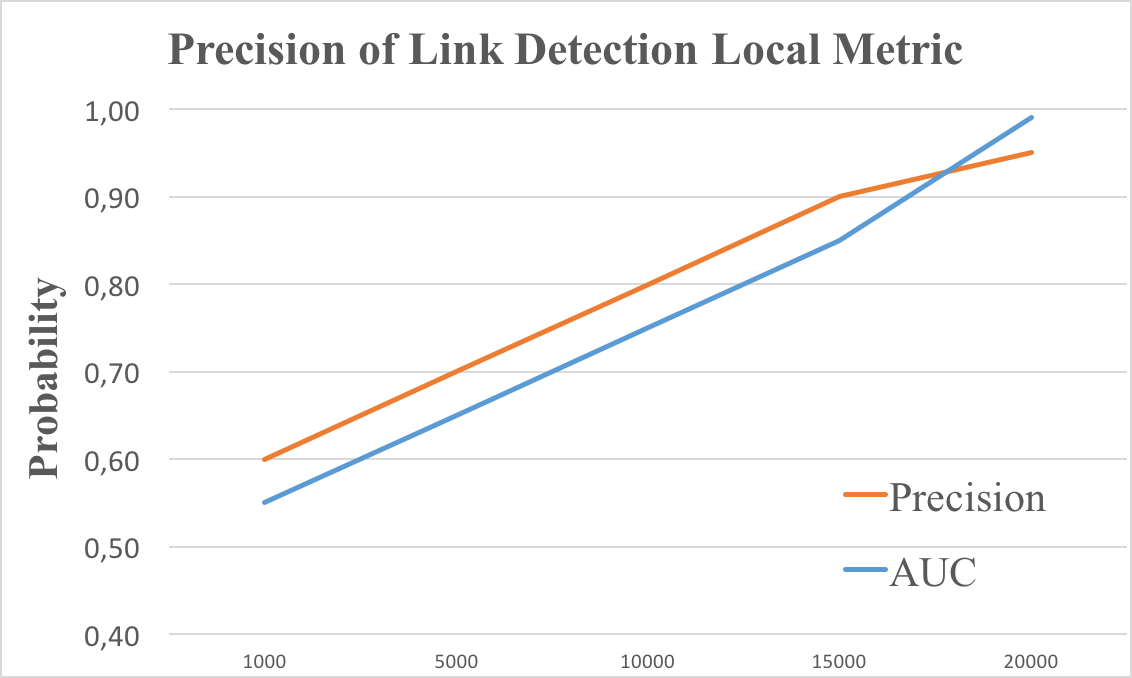
\includegraphics[width=0.48\textwidth]{graphs/graph_detection.png}
%	\caption{Precision of local metric for link detection}
%	\label{fig:graph-detection}
%\end{figure}

%\begin{figure}[!ht]
%	\centering
%	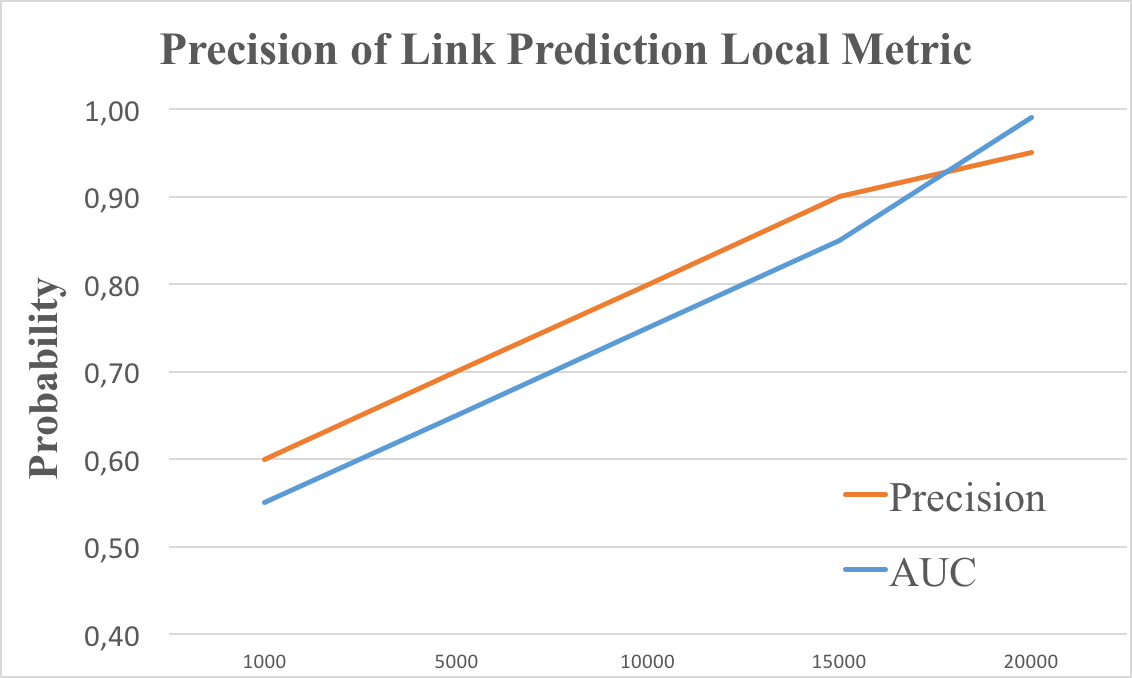
\includegraphics[width=0.48\textwidth]{graphs/graph_prediction.png}
%	\caption{Precision of local metric for link prediction}
%	\label{fig:graph-prediction}
%\end{figure}

\begin{table}[h]
	\centering
	\begin{tabular}{l l l l l}
	\toprule
	\textbf{Metric} & \textbf{CRM-10} & \textbf{CRM-15} & \textbf{BSN-10} & \textbf{BSN-15}\\
	\midrule
		CN & $0.99$ & $0.99$ & $0.99$ & $0.99$ \\
		SLT  & $0.99$ & $0.99$ & $0.99$ & $0.99$ \\
		JCR  & $0.99$ & $0.99$ & $0.99$ & $0.99$ \\
		SRS   & $0.99$ & $0.99$ & $0.99$ & $0.99$ \\
		HPI  & $0.99$ & $0.99$ & $0.99$ & $0.99$ \\
		HDI  & $0.99$ & $0.99$ & $0.99$ & $0.99$ \\
		LHN1  & $0.99$ & $0.99$ & $0.99$ & $0.99$ \\
		PA  & $0.99$ & $0.99$ & $0.99$ & $0.99$ \\
		AA  & $0.99$ & $0.99$ & $0.99$ & $0.99$ \\
		RA  & $0.99$ & $0.99$ & $0.99$ & $0.99$ \\
		NRA  & $0.99$ & $0.99$ & $0.99$ & $0.99$ \\
		TA  & $0.99$ & $0.99$ & $0.99$ & $0.99$ \\
		NTA  & $0.99$ & $0.99$ & $0.99$ & $0.99$ \\
	\bottomrule
	\end{tabular}
	\label{tab:auc-detection}
	\caption{AUC for link detection.}
\end{table}

\begin{table}[h]
	\centering
	\begin{tabular}{l l l l l}
	\toprule
	\textbf{Metric} & \textbf{CRM-10} & \textbf{CRM-15} & \textbf{BSN-10} & \textbf{BSN-15}\\
	\midrule
		CN & $0.99$ & $0.99$ & $0.99$ & $0.99$ \\
		SLT  & $0.99$ & $0.99$ & $0.99$ & $0.99$ \\
		JCR  & $0.99$ & $0.99$ & $0.99$ & $0.99$ \\
		SRS   & $0.99$ & $0.99$ & $0.99$ & $0.99$ \\
		HPI  & $0.99$ & $0.99$ & $0.99$ & $0.99$ \\
		HDI  & $0.99$ & $0.99$ & $0.99$ & $0.99$ \\
		LHN1  & $0.99$ & $0.99$ & $0.99$ & $0.99$ \\
		PA  & $0.99$ & $0.99$ & $0.99$ & $0.99$ \\
		AA  & $0.99$ & $0.99$ & $0.99$ & $0.99$ \\
		RA  & $0.99$ & $0.99$ & $0.99$ & $0.99$ \\
		NRA  & $0.99$ & $0.99$ & $0.99$ & $0.99$ \\
		TA  & $0.99$ & $0.99$ & $0.99$ & $0.99$ \\
		NTA  & $0.99$ & $0.99$ & $0.99$ & $0.99$ \\
	\bottomrule
	\end{tabular}
	\label{tab:auc-prediction}
	\caption{AUC for link prediction.}
\end{table}	
     
%\begin{figure}
%	\centering
%	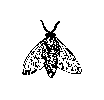
\includegraphics{./fig/fly}
%	\caption{AUC and Precision indices for link detection metric, considering both a criminal and a social network dataset.}
%	\label{fig:performance-detection}
%\end{figure}

%\begin{figure}
%	\centering
%	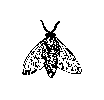
\includegraphics{./fig/fly}
%	\caption{AUC and Precision indices for link prediction metric, considering both a criminal and a social network dataset.}
%	\label{fig:performance-prediction}
%\end{figure}

% DA INSERIRE
%Formally, for two istants $t$ and $t' > t$, we denote $G[t,t']$ the subgraph of G consisting of all edges with a timestamp between $t$ and $t'$. Identified four times: $t_{0}, t'_{0}, t_{1}, t''_{1}$, with $t_{0}<t'_{0}<t_{1}<t'_{1}$, we refer to $[t_{0},t'_{0}]$ as the \textit{training interval} and $[t_{1},t'_{1}]$ as the \textit{test interval}. Applying a \textit{prediction algorithm} on the graph obtained after the training interval, as $G[t_{0},t'_{0}]$, we want to make a prediction on the edges that will be present in the graph $G[t_{1},t'_{1}]$ and not present in $G[t_{0},t'_{0}]$\cite{Liben-Nowell}.
%In this work, the notions of training interval and test interval, are provided with the only purpose to test the algorithm that will be presented in the following. After all, this application produce an output of links mining in real time: in which each instant $t\textsuperscript{*}>t_{0}$ identifies a graph $G[t_{0},t\textsuperscript{*}]$ on which to execute the algorithm. More details about the real time processing are explained in Section \ref{sec:architecture}.

%Notice that, in this work we assume that the graph is connected, therefore each pair of nodes is connected by a path. If we had in the case of a not connected graph, with a large connected component, as \textit{giant component}, and other small size connected components, the accuracy would be distorted by different \textit{density} of edges in a connected components.

\section{Further improvements}
\label{sec:further-improvements}

The application of big data analytics on criminal networks has a disruptive potential, opening new challenges for the field of social network analysis.
The proposed metrics meet the critical requirements, showing satisfactory results, but can certainly be improved. 
First of all, a scalable quasi-local extension of these metrics should be investigated to make them more flexible.
Then, their main limitation concerns the impossibility to mine links on networks made up of more than one connected components. 

A statistical approach could certainly overcome some of the limitations affecting structural metrics. In fact, their main limitation concerns the impossibility to mine links on criminal networks made up of more than one connected components.  
The criminological context is in line with the studies on traffic matrix estimation on IP networks  \cite{medina2002traffic,benameur2004traffic,papagiannaki2004distributed}. 
For instance, there could be an hidden link between two nodes, if the traffic matrix identifies a strict correlation between the outgoing and ingoing traffic from one another. 
The correlation could be detected by the traffic matrix decomposition techniques \cite{elgamal2015analysis,jiang2015covariance}. 
In this sense, the design of efficient data stream processing algorithms for the decomposition of sparse matrices will play a key role in the criminological domain.
\section{Conclusions}
\label{sec:conclusions}

The application of Big Data analytics on criminal networks has a disruptive potential for the data-driven fight against the organized crime, opening new challenges for the field of social network analysis. In this context it is necessary to develop new models for social networks analytics, ready to be deployed in a data stream environment. 

In this work we defined three new metrics for link detection and prediction in an evolving criminal network.
%
Furthermore, we proposed an algorithm to deploy both the new and the traditionally adopted metrics in a data stream environment.
%
The experiments were aimed at comparing traditional and new metrics and the proposed new ones in detecting and predicting criminal patterns, leveraging our data stream algorithm. 
%
The experimental results showed that the new metrics we proposed can reach an accuracy that is competitive with the traditional ones, both in detection and prediction.

% FUTURE WORK

The proposed models met the real-time and accuracy requirements, showing satisfying results, but can certainly be improved, as follows.
%
First of all, a stream-ready quasi-local extension of these metrics should be investigated to make them more flexible. 
%
The difficulty of this extension lies in the combinatorial explosion of metrics updates due to the bigger set of feature to examine.
%
A heuristic, possibly supported by in-memory caching features, could further improve the scalability of such an extension.

Another limitation concerns the impossibility to mine links on networks made up of more than one connected components. The native locality of the considered metrics, imposes such a limit by construction.
%
A statistical approach could overcome this limitation by allowing links mining on criminal networks containing more than one connected component. 


%*******************************************************************************
% Bibliography
%*******************************************************************************
\bibliographystyle{IEEEtran}
\bibliography{./ref/biblio}

\end{document}
